%%%%%%%%%%%%%%%%%%%%%%%%%%%%%%%%%%%%%%%%%
% Journal Article
% LaTeX Template
% Version 1.4 (15/5/16)
%
% This template has been downloaded from:
% http://www.LaTeXTemplates.com
%
% Original author:
% Frits Wenneker (http://www.howtotex.com) with extensive modifications by
% Vel (vel@LaTeXTemplates.com)
%
% License:
% CC BY-NC-SA 3.0 (http://creativecommons.org/licenses/by-nc-sa/3.0/)
%
%%%%%%%%%%%%%%%%%%%%%%%%%%%%%%%%%%%%%%%%%

%----------------------------------------------------------------------------------------
%	PACKAGES AND OTHER DOCUMENT CONFIGURATIONS
%----------------------------------------------------------------------------------------

\documentclass[twoside,twocolumn]{article}

\usepackage{blindtext} % Package to generate dummy text throughout this template 

\usepackage{hyperref}
\hypersetup{
    colorlinks=true,
    linkcolor=blue,
    filecolor=magenta,      
    urlcolor=cyan,
}

\usepackage[sc]{mathpazo} % Use the Palatino font
\usepackage[T1]{fontenc} % Use 8-bit encoding that has 256 glyphs
\linespread{1.05} % Line spacing - Palatino needs more space between lines
\usepackage{microtype} % Slightly tweak font spacing for aesthetics
\usepackage[utf8]{inputenc}

\usepackage[portuguese]{babel} % Language hyphenation and typographical rules

\usepackage[hmarginratio=1:1,top=32mm,columnsep=20pt]{geometry} % Document margins
\usepackage[hang, small,labelfont=bf,up,textfont=it,up]{caption} % Custom captions under/above floats in tables or figures
\usepackage{booktabs} % Horizontal rules in tables

\usepackage{lettrine} % The lettrine is the first enlarged letter at the beginning of the text
\usepackage{float}
\usepackage{enumitem} % Customized lists
\setlist[itemize]{noitemsep} % Make itemize lists more compact

\usepackage{abstract} % Allows abstract customization
\renewcommand{\abstractnamefont}{\normalfont\bfseries} % Set the "Abstract" text to bold
\renewcommand{\abstracttextfont}{\normalfont\small\itshape} % Set the abstract itself to small italic text
%\usepackage[shortlabels]{enumitem}
\usepackage{enumitem}
\usepackage{titlesec} % Allows customization of titles
\renewcommand\thesection{\Roman{section}} % Roman numerals for the sections
\renewcommand\thesubsection{\roman{subsection}} % roman numerals for subsections
\titleformat{\section}[block]{\large\scshape\centering}{\thesection.}{1em}{} % Change the look of the section titles
\titleformat{\subsection}[block]{\large}{\thesubsection.}{1em}{} % Change the look of the section titles

\usepackage{fancyhdr} % Headers and footers
\pagestyle{fancy} % All pages have headers and footers
\fancyhead{} % Blank out the default header
\fancyfoot{} % Blank out the default footer
\fancyhead[C]{MO443 $\bullet$ Junho 2019 $\bullet$ Relatório 05} % Custom header text
\fancyfoot[RO,LE]{\thepage} % Custom footer text

\usepackage{titling} % Customizing the title section

\usepackage{hyperref} % For hyperlinks in the PDF

\usepackage{graphicx}
\usepackage{subfigure}

\usepackage{mathtools}
\DeclarePairedDelimiter\floor{\lfloor}{\rfloor}
%----------------------------------------------------------------------------------------
%	TITLE SECTION
%----------------------------------------------------------------------------------------

\setlength{\droptitle}{-4\baselineskip} % Move the title up

\pretitle{\begin{center}\Huge\bfseries} % Article title formatting
\posttitle{\end{center}} % Article title closing formatting
\title{Relatório - Trabalho 05 \\ \Large MO443 - Introdução ao Processamento de Imagem Digital} %
%\subtitle{qsdqwdqwd} %Article title
\author{%
\textsc{Vinicius Teixeira de Melo - RA: 230223} \\[1ex] % Your name
\normalsize Universidade Estadual de Campinas \\ % Your institution
\normalsize \href{mailto:viniciusteixeira@liv.ic.unicamp.br}{viniciusteixeira@liv.ic.unicamp.br} % Your email address
%\and % Uncomment if 2 authors are required, duplicate these 4 lines if more
%\textsc{Jane Smith}\thanks{Corresponding author} \\[1ex] % Second author's name
%\normalsize University of Utah \\ % Second author's institution
%\normalsize \href{mailto:jane@smith.com}{jane@smith.com} % Second author's email address
}
\date{\today} % Leave empty to omit a date
\renewcommand{\maketitlehookd}{%
%\begin{abstract}
%\noindent \blindtext % Dummy abstract text - replace \blindtext with your abstract text
%\end{abstract}
}

%----------------------------------------------------------------------------------------

\begin{document}

% Print the title
\maketitle

%----------------------------------------------------------------------------------------
%	ARTICLE CONTENTS
%----------------------------------------------------------------------------------------

\section{Especificação do Problema}

O objetivo deste trabalho é aplicar técnicas de agrupamento de dados (ou seja, técnicas de aprendizado de máquina não supervisionado) para reduzir (quantizar) o número de cores de uma imagem colorida, procurando manter a qualidade da aparência geral da imagem de entrada.

Os principais passos do processo de geração da imagem quantizada são:

\begin{enumerate}
	\item ler a imagem colorida de entrada.
	\item aplicar a técnica \textit{k-means} de agrupamento de dados para encontrar grupos de cores mais representativas.
	\item salvar dicionário (\textit{codebook}) gerado pela técnica de agrupamento, ou seja, os centros dos grupos e os rótulos correspondentes a cada pixel da imagem.
	\item reconstruir a imagem com cores reduzidas a partir do dicionário armazenado.
\end{enumerate}

No passo (2), explore diferentes números de cores, por exemplo, 16, 32, 64 ou 128, para quantizar as imagens. Diferentes técnicas de agrupamento de dados também podem ser avaliadas.

A fundamentação e resolução deste trabalho estão descritas nas seções seguintes.

%------------------------------------------------

\section{Entrada de Dados}

O código fonte criado para a execução de todas as tarefas está no notebook \textbf{Trabalho 05.ipynb}. O código foi criado para aceitar imagens coloridas em diversos formatos, como exemplo: \textit{PNG} (\textit{Portable Network Graphics}), \textit{JPG} (\textit{Joint Photographic Group}), entre outros.

Para executar o notebook, basta iniciar o ambiente \textit{Jupyter Notebook}, abrir o notebook \textbf{Trabalho 05.ipynb} e executar as células em ordem. Todo o algoritmo foi implementado na linguagem Python na versão 3.6.

As imagens de entrada utilizadas nso testes dos algoritmos foram retiradas da página do prof. Hélio Pedrini: \href{http://www.ic.unicamp.br/~helio/imagens_coloridas/}{Imagens}. Na pasta \textbf{imgs/} estão as imagens coloridas utilizadas nos testes: \textbf{baboon.png} (512 x 512 \textit{pixels}) e \textbf{monalisa.png} (256 x 256\textit{pixels}).

\begin{figure}[H]
\begin{center}
	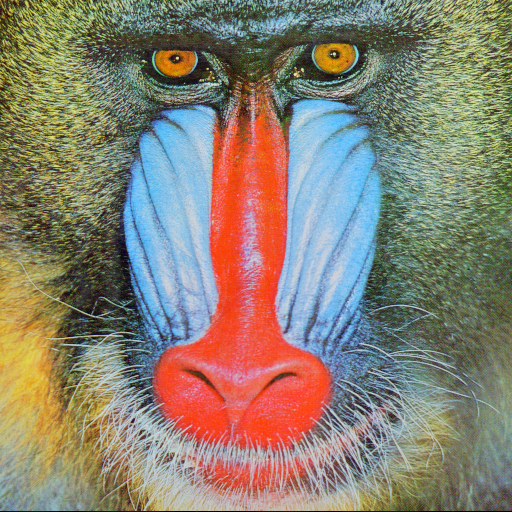
\includegraphics[height=6cm]{figures/baboon.png}
\caption{baboon.png} \label{baboon}
\end{center}
\end{figure}

\begin{figure}[H]
\begin{center}
	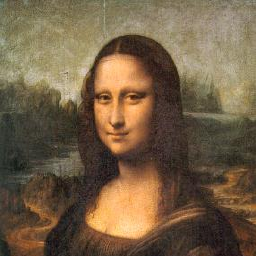
\includegraphics[height=6cm]{figures/monalisa.png}
\caption{monalisa.png} \label{monalisa}
\end{center}
\end{figure}

%------------------------------------------------

\section{Dependências e Códigos}

As bibliotecas utilizadas neste trabalho foram:

\begin{table}[H]
\begin{center}
\begin{tabular}{|l|l|}
\hline
\textbf{Biblioteca} & \textbf{Versão} \\ \hline
numpy               & 1.16.2          \\ \hline
cv2                 & 3.4.2           \\ \hline
matplotlib          & 3.0.3           \\ \hline
scikit-learn        & 0.20.3	      \\ \hline
warnings            & 2.1             \\ \hline
\end{tabular}
\end{center}
\end{table}

A leitura das imagens foi realizada utilizando uma função do \textbf{matplotlib} \cite{b3} chamada \textbf{pyplot.imread()}, a qual nescessita apenas do caminho da imagem, já que queremos as informações das imagens assim como estão.

Foi criada uma função para plotar os resultados finais utilizando também uma função do \textbf{matplotlib} chamada \textbf{pyplot.imshow()}. Nos passos (2) e (3) foram utilizadas funções da biblioteca \textbf{sklearn}, como \textbf{KMeans()} para a criação do modelo de agrupamento e \textbf{shuffle()} para a inicialização da amostragem das cores.

Por fim, no passo (4) foram utilizados os resultados dos passos anteriores para a recriação das imagens com a quantização de cores alteradas. Vale lembrar também que, inicialmente, as imagens foram transformadas de \textbf{uint8} para \textbf{float64} e seus níveis de intensidade foram normalizados para o intervalo [0,1], ao dividir por 255. E, no final, tiveram seus valores transformados novamente ao multiplicar os níveis de intensidade por 255.

%------------------------------------------------

\section{Fundamentação}

\subsection{Agrupamento de dados}

O clustering ou agrupamento de dados é o conjunto de técnicas de prospeção de dados que visa fazer agrupamentos automáticos de dados segundo o seu grau de semelhança. O critério de semelhança faz parte da definição do problema e, dependendo, do algoritmo. A cada conjunto de dados resultante do processo dá-se o nome de grupo, aglomerado ou agrupamento (\textit{cluster}) \cite{b4}.

Normalmente o usuário do sistema deve escolher a priori o número de grupos a serem detectados. Alguns algoritmos mais sofisticados pedem apenas o número mínimo, outros tem a capacidade de subdividir um grupo em dois. Quando se tem um conjunto de objetos é natural olhar para eles tentando perceber o quão semelhantes ou diferentes eles são uns dos outros. Uma abordagem comum consiste em definir uma função de distância entre os objetos, com a interpretação de que objetos a uma distância menor são mais semelhantes uns aos outros.

\subsubsection{KMeans}

\textit{KMeans} é um método de quantização vetorial, originalmente aplicado para processamento de sinais, que é popular para análise de agrupamentos em \textit{data mining}. Essa técnica tem como objetivo particionar um conjunto de $n$ objetos em $k$ \textit{clusters}, nos quais cada objeto pertence ao \textit{cluster} com a média mais próxima.

O problema é definido formalmente como: Dado um conjunto de observações ($x_{1}, x_{2}, ..., x_{n}$) onde cada observação é um vetor real de $d$ dimensões, \textit{kmeans} particiona as $n$ observações em $k$ conjuntos $S = \{S_{1}, S_{2}, ..., S_{k}\}$ de tal forma que minimize a soma dos erros quadráticos.
 
%------------------------------------------------

\section{Saída de Dados}

As imagens resultantes foram salvas dentro da pasta \textbf{resultados/} utilizando uma função da biblioteca \textbf{matplotlib} chamada \textbf{pyplot.imsave()} \cite{b3}.

O formato dos nomes de saída estão da seguinte forma: primeiramente é o nome da imagem de entrada (baboon ou monalisa) concatenado com ''\_'' e o número de \textit{clusters} utilizados na criação do modelo de agrupamento \textit{KMeans}.

%------------------------------------------------

\section{Resultados e Discussões}

Nesta seção são apresentados os resultados obtidos após os passos descritos anteriormente e uma discussão sobre cada resultado.

A Figura~\ref{quant_16} apresenta o resultado da aplicação da técnica de agrupamento de cores, utilizando 16 \textit{clusters}. Podemos observar que, como a quantidade de cores é muito reduzida, as imagens resultantes contém regiões que se tornaram homogêneas, tendo assim muitas perdas de informações acerca dos detalhes contidos nas imagens.

\begin{figure}[h]
\begin{center}
	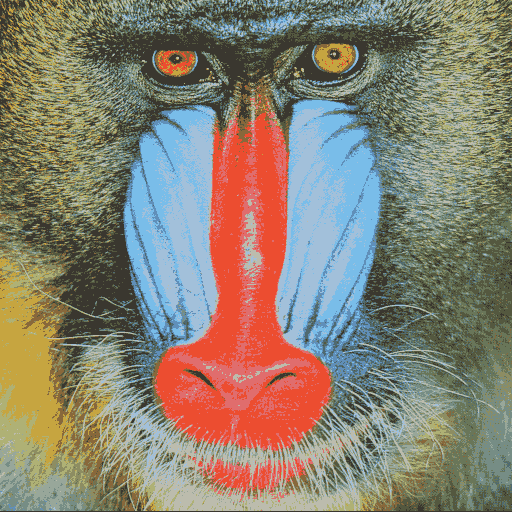
\includegraphics[height=6cm]{figures/baboon_16.png}
	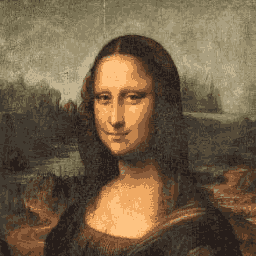
\includegraphics[height=6cm]{figures/monalisa_16.png}
\caption{Resultado da quantização com 16 cores.} \label{quant_16}
\end{center}
\end{figure}

A Figura~\ref{quant_32} apresenta agora o resultado utilizando 32 \textit{clusters}. Podemos observar que, diferente do resultado anterior, agora é possível notar mais detalhes nas imagens e as áreas homogêneas se tornaram bem menores, por conta de estarmos utilizando uma quantidade maior de cores para quantizar as imagens.

\begin{figure}[h]
\begin{center}
	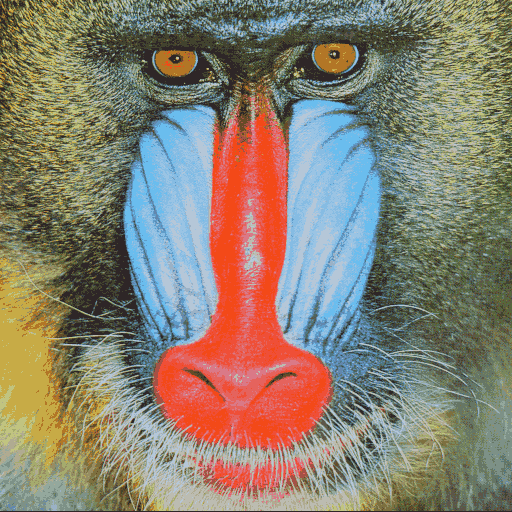
\includegraphics[height=6cm]{figures/baboon_32.png} \quad
	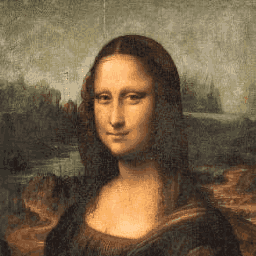
\includegraphics[height=6cm]{figures/monalisa_32.png}
\caption{Resultado da quantização com 32 cores.} \label{quant_32}
\end{center}
\end{figure}

A Figura~\ref{quant_64} mostra os resultados obtidos utilizando quantização com 64 \textit{clusters}. Agora, já não é possível fazer uma distinção grande para o resultado com 32 \textit{clusters}, pois o olho humano não distingue esse nível de detalhes. Mas podemos perceber que as regiões que estavam homogêneas no resultado anterior não existem mais, assim, o nível de detalhes foi elevado.

\begin{figure}[h]
\begin{center}
	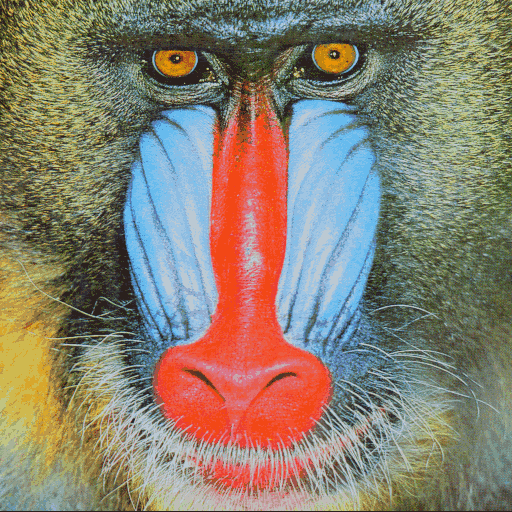
\includegraphics[height=6cm]{figures/baboon_64.png} \quad
	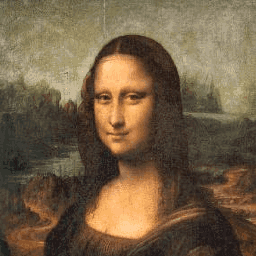
\includegraphics[height=6cm]{figures/monalisa_64.png}
\caption{Resultado da quantização com 64 cores.} \label{quant_64}
\end{center}
\end{figure}

Por fim, a Figura~\ref{quant_128} apresenta os resultados obtidos utilizando a técnica de agrupamento com 128 \textit{clusters}. Já não é mais possível distinguir diferenças para o resultado anterior (64 \textit{clusters}), o que nos diz que está próximo ou já chegou na quantidade de cores utilizadas na imagem anterior, assim, o agrupamento não altera mais as imagens de entrada.

\begin{figure}[h]
\begin{center}
	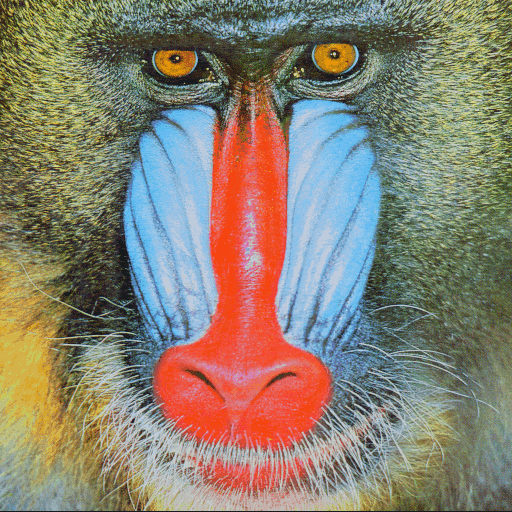
\includegraphics[height=6cm]{figures/baboon_128.png} \quad
	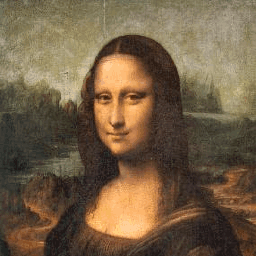
\includegraphics[height=6cm]{figures/monalisa_128.png}
\caption{Resultado da quantização com 128 cores.} \label{quant_128}
\end{center}
\end{figure}

%------------------------------------------------

\section{Conclusão}

Podemos concluir que os resultados obtidos com as aplicações da técnica de quantização de imagem \textit{KMeans} se mostrou eficiente e efetivo, apresentando resultados satisfatórios quanto a especificação do trabalho e se mostrou razoável para este objetivo, assim, consolida ainda mais os conceitos vistos em sala de aula.

%----------------------------------------------------------------------------------------
%	REFERENCE LIST
%----------------------------------------------------------------------------------------

\begin{thebibliography}{99} % Bibliography - this is intentionally simple in this template

\bibitem{b1} Documentation of scikit-learn. \href{https://scikit-learn.org/stable/documentation.html}{https://scikit-learn.org/stable/documentation.html} Acesso em: 22/06/2019.

\bibitem{b2} Pedrini, Hélio, and William Robson Schwartz. Análise de imagens digitais: princípios, algoritmos e aplicações. Thomson Learning, 2008.

\bibitem{b3} Matplotlib Version 3.0.3 \href{https://matplotlib.org/contents.html}{https://matplotlib.org/contents.html} Acesso em: 22/06/2019.

\bibitem{b4} Clustering \href{https://pt.wikipedia.org/wiki/Clustering}{https://pt.wikipedia.org/wiki/Clustering} Acesso em: 22/06/2019.
 
\end{thebibliography}

%----------------------------------------------------------------------------------------

\end{document}
